\documentclass[letterpaper,10pt]{article}

\usepackage{enumitem}
\usepackage{titling}
\usepackage{listings}
\usepackage{url}
\usepackage{hyperref}
\usepackage{setspace}
\usepackage{subfig}
\usepackage{sectsty}
\usepackage{pdfpages}
\usepackage{colortbl}
\usepackage{multirow}
\usepackage{multicol}
\usepackage{relsize}
\usepackage{amsmath}
\usepackage{wasysym}
\usepackage{fancyvrb}
\usepackage[yyyymmdd]{datetime}
\usepackage{amsmath,amssymb,amsthm,graphicx,xspace}
\usepackage[titlenotnumbered,noend,noline]{algorithm2e}
\usepackage[compact]{titlesec}
\usepackage{XCharter}
\usepackage[T1]{fontenc}
\usepackage[scaled]{beramono}
\usepackage[normalem]{ulem}
\usepackage{booktabs}
\usepackage{tikz}
\usetikzlibrary{arrows,automata,shapes,trees,matrix,chains,scopes,positioning,calc}
\tikzstyle{block} = [rectangle, draw, fill=blue!20,
text width=2.5em, text centered, rounded corners, minimum height=2em]
\tikzstyle{bw} = [rectangle, draw, fill=blue!20,
text width=4em, text centered, rounded corners, minimum height=2em]

\definecolor{namerow}{cmyk}{.40,.40,.40,.40}
\definecolor{namecol}{cmyk}{.40,.40,.40,.40}
\renewcommand{\dateseparator}{-}

\let\LaTeXtitle\title
\renewcommand{\title}[1]{\LaTeXtitle{\textsf{#1}}}

\lstset{basicstyle=\footnotesize\ttfamily,breaklines=true}

\newcommand{\handout}[5]{
	\noindent
	\begin{center}
		\framebox{
			\vbox{
				\hbox to 5.78in { {\bf SE 350: Operating Systems } \hfill #2 }
				\vspace{4mm}
				\hbox to 5.78in { {\Large \hfill #4  \hfill} }
				\vspace{2mm}
				\hbox to 5.78in { {\em #3 \hfill \today} }
			}
		}
	\end{center}
	\vspace*{4mm}
}

\newcommand{\lecture}[3]{\handout{#1}{#2}{#3}{Lecture#1}}
\newcommand{\tuple}[1]{\ensuremath{\left\langle #1 \right\rangle}\xspace}

\newcommand{\Rplus}{\protect\hspace{-.1em}\protect\raisebox{.35ex}{\smaller{\smaller\textbf{+}}}}
\newcommand{\Cpp}{\mbox{C\Rplus\Rplus}\xspace}


\addtolength{\oddsidemargin}{-1.000in}
\addtolength{\evensidemargin}{-0.500in}
\addtolength{\textwidth}{2.0in}
\addtolength{\topmargin}{-1.000in}
\addtolength{\textheight}{1.75in}
\addtolength{\parskip}{\baselineskip}
\setlength{\parindent}{0in}
\renewcommand{\baselinestretch}{1.5}
\newcommand{\term}{Winter 2023}
\newcommand{\termnumeric}{1231}

\singlespace


\begin{document}

\lecture{ 32 --- Disk Scheduling }{\term}{Jeff Zarnett}

\section*{Disk Scheduling}
The disk is a very slow device, as far as the CPU is concerned, so we want to avoid going to disk, if it can be helped, whenever possible. We will examine the hardware behind magnetic hard disks and see why they are so slow and consider several algorithms that could be used to speed up operations.

I'm going to imagine that you got a solid-state drive (SSD) in your computer when you purchased it. But back before those were common, the mass and permanent storage of data in your system was on a magnetic hard disk. Due to the physical nature of how disk drives work, there is an associated delay with moving to a new location and reading the data there. Thus, we would like to devise efficient schedules for reading and writing, just as in the example from earlier, we wished to avoid going back-and-forth when completing a set of weekly errands.

We will exclude SSDs from consideration here. SSDs do not contain moving disk heads or spinning platters. Thus, an algorithm to schedule the optimal movement of the disk heads is not relevant. Read access times from the SSD are consistent and uniform even if data is being requested from random locations. So, the SSD disk scheduling algorithm can be as simple as first-come, first-served.

That prompts the question: why bother learning about this if magnetic drives are going away? The first is that while magnetic drives might be on the way out, they're not dead yet and many systems still use them, including large databases. The other is that disks are a convenient example, but not the only I/O device that needs to seek around to read and write data, so what we examine here may be applicable to other sorts of devices too.

The diagram below is a quick overview of what hard drives look like internally. Hard drives come in carefully sealed packages and if you open one (please don't; this is very bad for your ability to read data from it) it looks something like this:

\begin{center}
	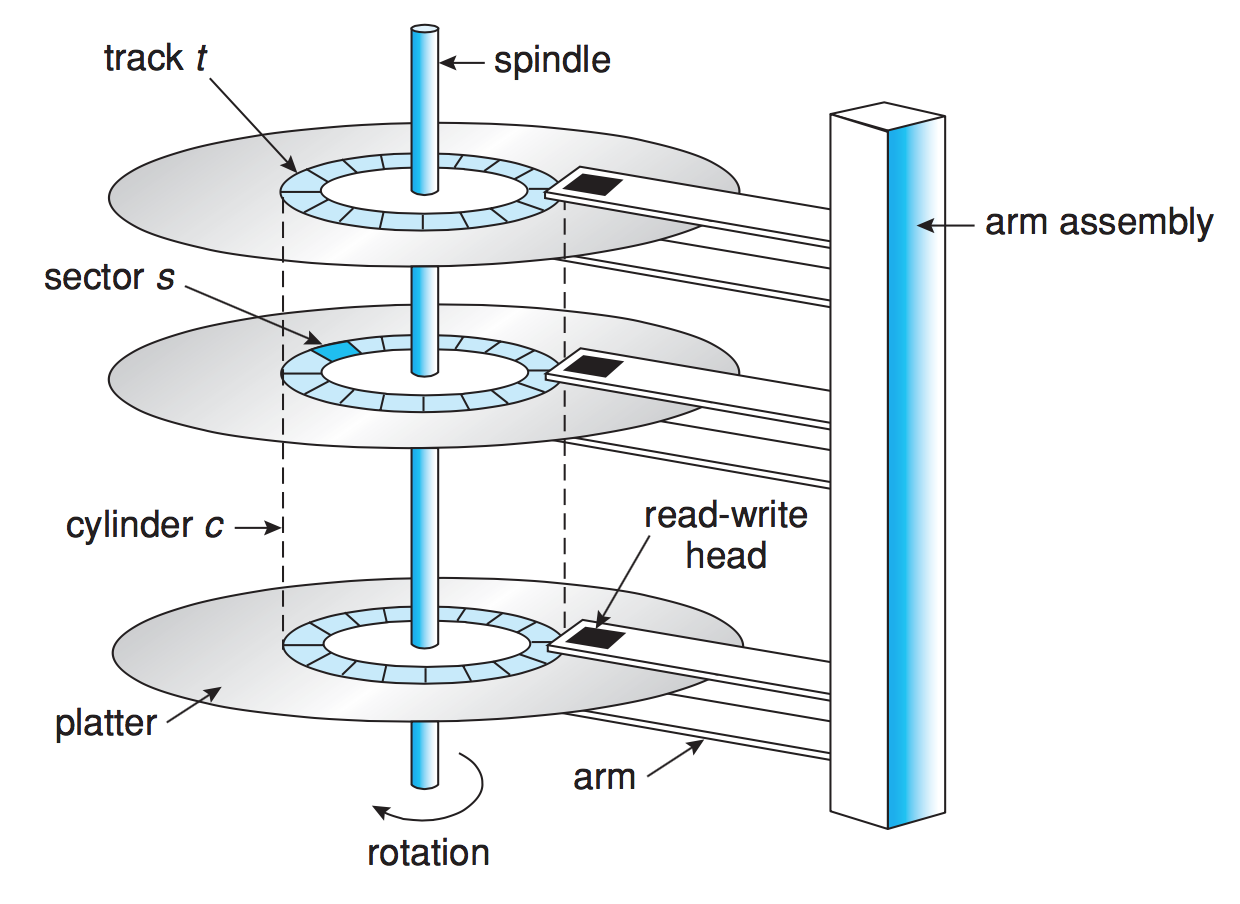
\includegraphics[width=0.6\textwidth]{images/disk-hardware.png}\\
	Moving-head disk mechanism~\cite{osc}.
\end{center}

A read-write head is suspended a very small distance above the surface of each platter and reads or writes data directly beneath it. This is why they are carefully sealed: if a bit of dust lands on the platter, the read-write head can run into it (which is bad). It gets even worse if a disk head makes contact with the platter: this is called a head crash and it tends to permanently destroy data. The platter surface is divided logically into different circular tracks, which are respectively divided up into sectors (blocks). A set of tracks stacked vertically is called a column. When the disk is in use, a motor spins the platters at high speed and another one manipulates the positions of the arm.

The performance of the disk can be broken down into two values. The first is the \textit{transfer rate}; the speed at which data can be moved from the disk to the computer or vice-versa. The other is the \textit{random-access time}; how long it takes to get to a particular piece of data. The random access time itself is broken down into the \textit{seek time}, how long it takes to move the disk arm to the right position, and the \textit{rotational latency}, how long it takes to rotate the platters to the right position. Seek times and rational latencies tend to run in the millisecond range~\cite{osc}.

\begin{center}
	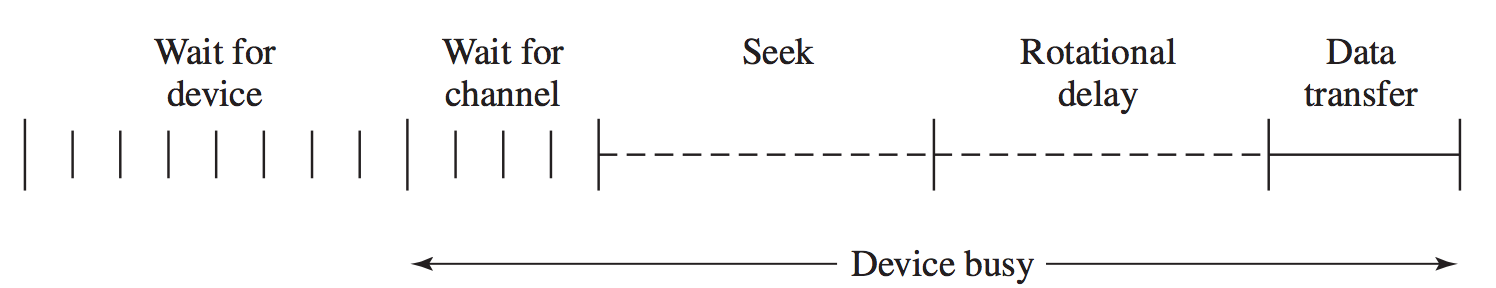
\includegraphics[width=0.7\textwidth]{images/disk-transfer-time.png}\\
	Disk I/O transfer timing~\cite{osi}.
\end{center}

The total average access time, $T_{a}$, for a disk operation can be defined as~\cite{osi}:

\begin{center}
$T_{a} = T_{s} + \dfrac{1}{2r} + \dfrac{b}{rN}$
\end{center}
Where: $T_{s}$ is the average seek time, $r$ is the rotation speed (revolutions per second), $b$ is the number of bytes to be transferred, and $N$ is the number of bytes on a track.

\paragraph{Example.} Let's take an example from~\cite{osi} that illustrates just how much variance we can have in disk performance. In this scenario, the disk has an average seek time of 4~ms, a rotation speed of 7~500 RPM, and 512-byte sectors with 500 sectors per track. We want to read a file that is 2~500 sectors (a total of 1.28~MB). 

If the file is stored as compactly on disk as it can be, it is \textit{sequentially organized}: the file occupies all the sectors on 5 adjacent tracks. To read the first track, it will take 16~ms: 4~ms to seek, 4~ms rotational delay, and then 8~ms to read 500 sectors. Because the data is sequential, no additional seek time is necessary, so we just keep reading subsequent sectors which means only the rotational delay. Each additional track takes 12~ms (4~ms rotational delay + 8~ms to read it). Thus the total time is $16 + (4 \times 12)$ = 64~ms.

What if instead the data was randomly distributed on the disk and not sequential? The average seek and rotational delay times don't change. Reading one sector takes 0.016~ms. So each read of a sector will take a total of 8.016~ms ($4 + 4 + 0.016$). There are 2~500 sectors so the total is $2~500 \times 8.016 =$ 20~040~ms. 

20~000~ms - twenty full seconds to read 1.28~MB of data? Yes. Seriously. This speed would be considered utterly unacceptable by the users. So it is clear that the order in which sectors are read from the disk makes a huge difference. This suggests that decisions about how to store data on disk is extremely important. Not only is the placement important, but how we schedule the reads and writes.

\subsection*{Disk Scheduling}
We should introduce a final metric, the \textit{bandwidth}: the total number of bytes transferred, divided by the total time between the request for service and completion of the transfer. This is a measure of how much data is effectively transferred in a period of time. This is one of the measures we would like to improve, as well as the access time.

When a process needs to read from or write to the disk, the system call contains the following information~\cite{osc}:

\begin{enumerate}
	\item If the operation is a read or write.
	\item The disk address for the transfer.
	\item The memory address for the transfer.
	\item How much data to transfer (how many sectors).
\end{enumerate}

Nobody actually seriously advocates random scheduling, but it is a baseline against which to compare various scheduling algorithms. We can assess the various options based on their improvement relative to random scheduling. We could do disk accesses based on process priority, paying no attention to how (in)convenient it is from the perspective of the disk; the highest priority process's request gets serviced first. 

Similarly, if there is only one request for a read or write, there is not much of a decision to make. If the disk is otherwise idle, service that request, regardless of where it is. Assuming we are not going to choose the priority option and we have more than one operation to perform, we have some decisions to make.

\subsubsection*{First-Come, First-Served}
This algorithm, also sometimes called First-In, First-Out, is fair and simple, but does not necessarily provide the fastest service because no attempt is made to group, organize, or rearrange the requests.

Example: requests for I/O to/from cylinders: \{98, 183, 37, 122, 14, 124, 65, 67\}; the disk head begins at 53.

\begin{center}
	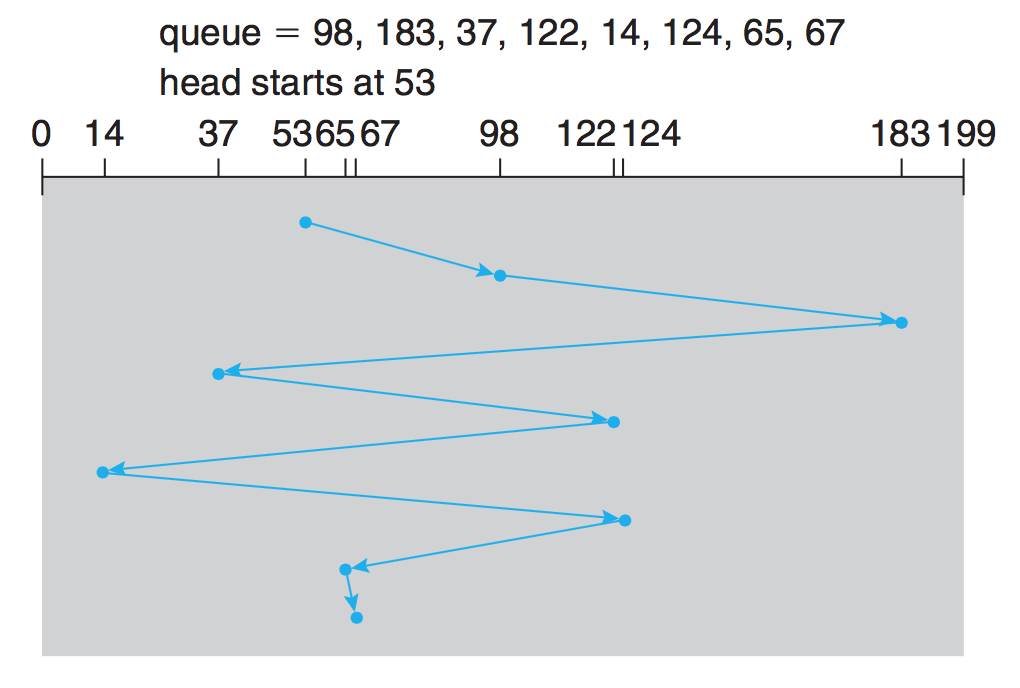
\includegraphics[width=0.5\textwidth]{images/disk-fcfs.png}\\
	FCFS disk scheduling~\cite{osc}.
\end{center}

So the disk head moves from 53 to 98, then 98 to 183, and so on, for a total movement of 640 cylinders. This example intentionally includes the sequence \{122, 14, 124\} to illustrate the problem: a wild swing back and forth over a long distance. It would be obviously better to do visit 122 and 124 after one another. 

\subsubsection*{Shortest Seek Time First}
Based on the idea that we want adjacent operations to take place consecutively, instead of just choosing the next item in the queue, choose the request with the least seek time from the current head position.

Using the same example as before, the closest request to the start position of 53 is cylinder 65. From there, 67 is next, then 37, 14, 98, 122, 124, and 183. Following this routine, the total head movement is 236 cylinders, a remarkable improvement over the 640 from before.

\begin{center}
	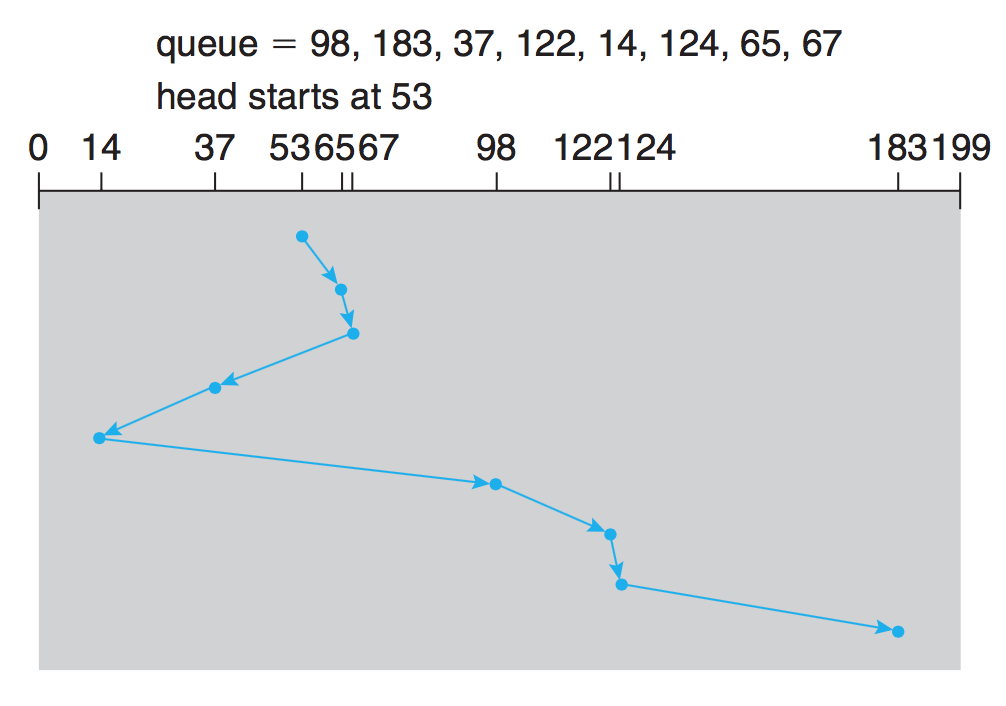
\includegraphics[width=0.5\textwidth]{images/disk-sstf.png}\\
	SSTF disk scheduling~\cite{osc}.
\end{center}

This routine is unfortunately subject to starvation. Suppose the disk head is at position 14. While it is there, a new request at 24 arrives, making the request at 98 wait. If enough low-numbered requests arrive to arrive during execution, a request at a high number may be put off, potentially indefinitely. The more requests occur, the more likely starvation is.

Though the SSTF algorithm is an improvement, it is not optimal. In the example, we would reduce the total amount of movement to 208 cylinders if we did the move from 53 to 37, even though it is not the closest, and then to 14, before moving to 65, 67, 98, 122, 124, and 183~\cite{osc}.

This algorithm provides for some spatial locality. If there are a number of requests that are located near one another on the disk, the SSTF algorithm takes advantage of this and will carry out all those requests relatively quickly.

\subsubsection*{SCAN Scheduling}
In the SCAN algorithm, instead of a ``zig-zag'' pattern where we might move in one direction and then immediately double back to another, such as 25 then 32, then 17, we move in one direction at a time until it reaches the ``end'' of the disk. After that, the direction is reversed. The SCAN algorithm is sometimes called the elevator algorithm, because it works like an elevator in a building; first all requests going up are serviced, then the elevator reverses direction and services all requests going down~\cite{osc}.

Let us assume the current direction of the head (starting at 53) is moving towards 0. So the algorithm will go to: 37, 14, then reverse direction and go to 65, 67, 98, 122, 124, and 183. If a request arrives just in front of the head (e.g, 129 arrives before 124 is serviced), it will be serviced virtually right away; if it is just after where the head has been (e.g., 123 after 124 has been serviced) it will wait until the direction reverses again. 

\begin{center}
	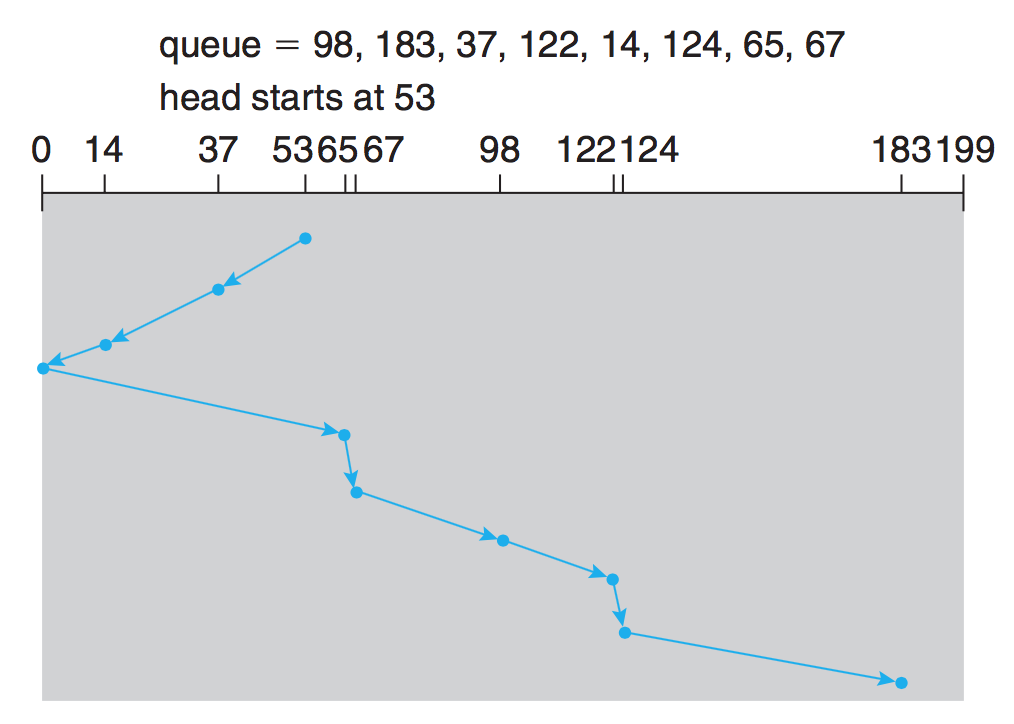
\includegraphics[width=0.5\textwidth]{images/disk-scan.png}\\
	SCAN disk scheduling~\cite{osc}.
\end{center}

Note that the SCAN policy does not take advantage of spatial locality as SSTF does. If the head has just moved from an area, it can be a long time before it returns to that area. Thus, if there are multiple accesses in the same area, they are likely to be at least partly spread out in time.

\subsubsection*{C-SCAN Scheduling}

An improvement on SCAN, known as C-SCAN is designed to exploit the fact that when the disk has just reached one end, most requests are likely at the other end of the disk (if they were nearby they would have been serviced already). So instead of reversing the direction and servicing requests on the way, jump back to the start of disk immediately and start at the beginning. It is called C-SCAN because C is for ``Circular''\footnote{C is also for cookie.}, as if the last cylinder just wraps around to the first.

\begin{center}
	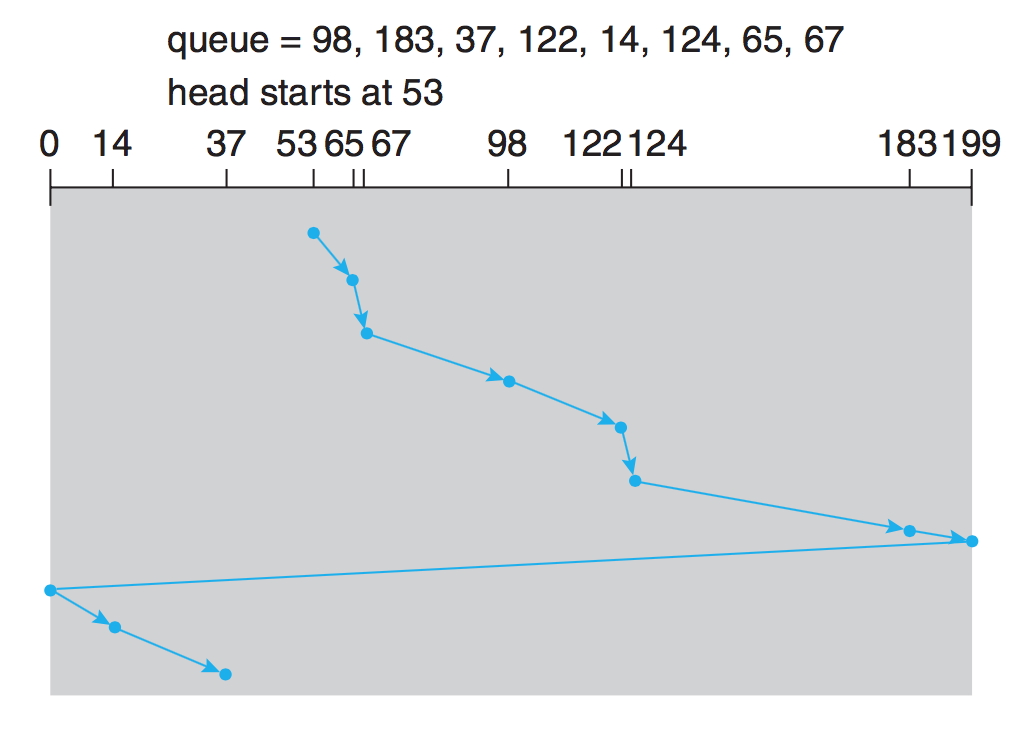
\includegraphics[width=0.5\textwidth]{images/disk-cscan.png}\\
	C-SCAN disk scheduling~\cite{osc}.
\end{center}

If the amount of time it takes to scan from the start to end of disk is $t$, the expected service interval for sectors at the periphery is $2t$ when using the SCAN algorithm. C-SCAN reduces this interval to approximately $t + s_{max}$ where $s_{max}$ is the maximum seek time~\cite{osi}.


\subsubsection*{LOOK Scheduling}
The SCAN and C-SCAN algorithms as described can be optimized in a little way: instead of going all the way to the end of disk every time, instead just go to the final request and only then reverse direction (or go back to the start). The names for this variant are LOOK and C-LOOK, respectively. 

\begin{center}
	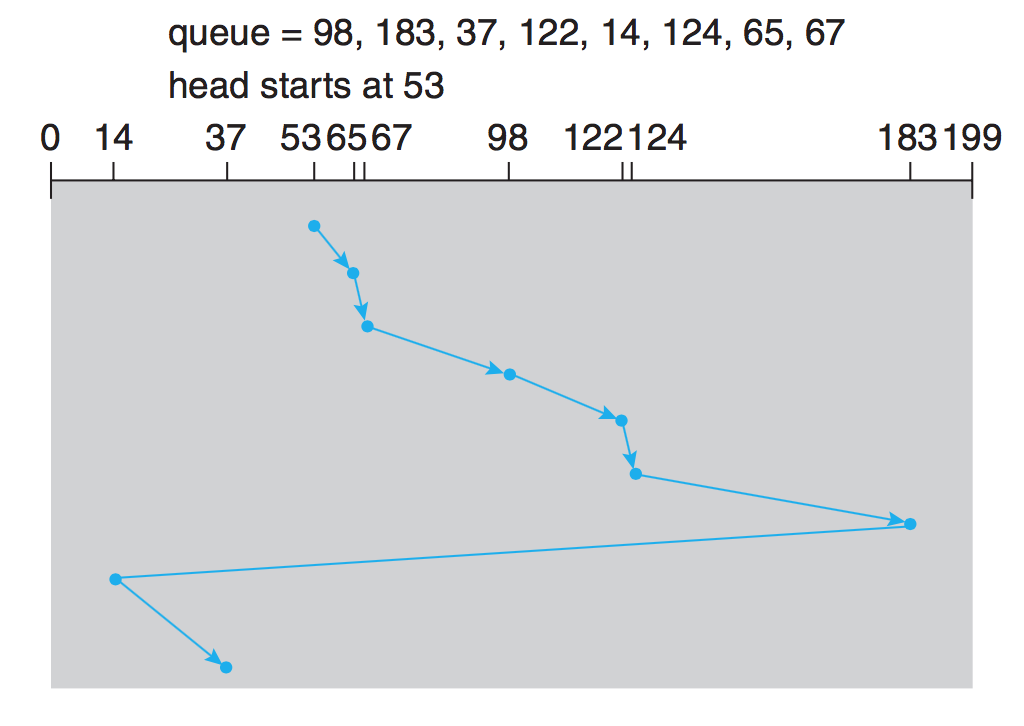
\includegraphics[width=0.5\textwidth]{images/disk-clook.png}\\
	C-LOOK disk scheduling~\cite{osc}.
\end{center}



\subsection*{Some More Details of Scheduling Algorithms}

Although we can probably agree that FCFS is not the best choice, how do we decide between the other options? The LOOK approach seems like it would prevent the starvation problem, which might otherwise would be an issue with SSTF. Although we expect that with the SCAN or C-SCAN algorithm, all requests get serviced, it could happen that a process is effectively starved or has to wait an inordinately long time because the request at the end of the disk is constantly postponed as more and more and more requests come in. 

A strategy to prevent this is a modification of the SCAN algorithm such that it has two queues for requests (think double buffering). While one queue is being emptied, the other is being filled. Thus, a request will not wait indefinitely; if the queue is of capacity $C$ then any particular read or write will wait, at most, $C$ accesses. The larger the value of $C$, the more the performance resembles SCAN; a smaller value of $C$ means behaviour is more like FCFS. The choice of $C$ is a trade off; we will sacrifice a bit of performance to increase the fairness~\cite{osi}.

The scheduling algorithms above consider only the seek times, and not the rotational latency, even though they can be about the same size. This is because it is very difficult for the OS to schedule for improved rotational latency, because the disk itself is responsible for the physical placement of the logical blocks. So, to make this a little easier, the hard disk controller takes on some of the scheduling options. The OS can provide to the controller a grouping of requests, and then the controller will figure out how to schedule them such that it takes into account the rotational latency as well as the seek time~\cite{osc}.

If the speed of disk reads and writes were the only thing to be concerned about, the operating system would probably not worry about disk scheduling and it would just be the job of the hard disk controller. However, the OS may have certain goals that should take precedence over the highest performance option. For example, loading a page into main memory might need to take priority over an application writing a file to disk. Higher priority processes, especially in real-time systems, should not be waiting (for too long at least) for lower priority processes' disk writes. So, under some circumstances, the operating system needs to manage the reads and writes and not just leave it up to the disk controller~\cite{osc}.


\bibliographystyle{alphaurl}
\bibliography{350}


\end{document}